\documentclass[mathserif]{beamer}
\usepackage[utf8]{inputenc}
\usepackage[english]{babel}
\usepackage[normalem]{ulem}

\usepackage{url}
\usepackage{hyperref}
\usepackage{fancyvrb}
\usepackage{csquotes}
\usepackage{upquote}
\usepackage{../lib/diagrams}

\usepackage{amsmath}
\usepackage{amssymb}
\usepackage{amsthm}
\usepackage{tikz}
\usetikzlibrary{matrix}

\newcommand{\catx}[1]{\mathbb{#1}}
\newcommand{\catC}{\catx{C}}
\newcommand{\catD}{\catx{D}}

\newcommand{\opcat}[1]{{#1}^{\text{op}}}
\newcommand{\Sets}{\mathbf{Sets}}
\newcommand{\Cat}{\mathbf{Cat}}
\newcommand{\Hask}{\mathbf{Hask}}

%% @TODO: invent some kid of inline 'code' style for this
\newcommand{\firstArr}{\texttt{first}}

%% @TODO: pick a 'math' style for arrow operations
\newcommand{\arrM}{\text{arr}}
\newcommand{\firstM}{\text{first}}
%% >>>, <<< are \ggg and \lll

\DefineVerbatimEnvironment{code}{Verbatim}{fontsize=\small,commandchars=\\\{\},codes={\catcode`$=3\catcode`_=8}}

\hypersetup{
    colorlinks,
    linkcolor=black,
    citecolor=black,
    filecolor=black,
    urlcolor=black
}


\usetheme{default}
\usecolortheme{default}
\usefonttheme{structuresmallcapsserif}
\setbeamertemplate{navigation symbols}{}

\usepackage{tikz}
\newenvironment{itemeyez}{\begin{itemize}%
    \setlength{\itemindent}{5em}}{%
    \end{itemize}}

\title{Cat Arrows}
\subtitle{What is a categorical semantics for arrows?}
\author[Vyšniauskas, Emerich]
{Ignas Vyšniauskas \and Johannes Emerich}
\institute{%
  ILLC \\
  Universiteit van Amsterdam
}
\date{November 1, 2013}
\subject{Computer Science}

\begin{document}

\frame{\titlepage}

\begin{frame}
    \frametitle{This is a presentation on Arrows.}
\end{frame}

\section{Context}
\begin{frame}
\frametitle{Liberating Programming from the ``von Neumann'' style}

\begin{itemize}
    \item John Backus' call for new language paradigm (1978)
    \begin{itemize}
        \item \emph{Functional} programming (``FP'') as combinatorial
              approach to program construction
        \item Construct programs in an algebra of programs
        \item Variables range over \emph{programs}, operations are \emph{on}
              programs (\emph{pointfree} style)
        \item Functional style: only one state transition per operation
    \end{itemize}
    \item Haskell as most popular language true to Backus' ideas
\end{itemize}
\end{frame}

\begin{frame}
\frametitle{Haskell is non-strict}

\begin{columns}[c]
    \begin{column}{.6\textwidth}
        \begin{itemize}
            \item Problem of functions in computing: non-termination
            \item \emph{Lift} all types by adding an \texttt{undefined} ($\bot$) bottom
                  element, lowest in information order
            \item Set $B = \{\textrm{True}, \textrm{False}\}$ lifted to $B_\bot
                  = B \cup \{\bot\}$
            \item Functions are $B_\bot \to B_\bot$
        \end{itemize}
    \end{column}
    \begin{column}{.4\textwidth}
        \begin{center}
        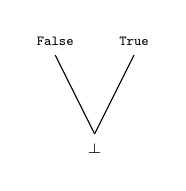
\begin{tikzpicture}
            \draw[font=\tiny] (0,0) node[below] {$\bot$} -- (0.5,1) node[above] {\texttt{True}};
            \draw[font=\tiny] (0,0) -- (-0.5,1) node[above] {\texttt{False}};
        \end{tikzpicture}
        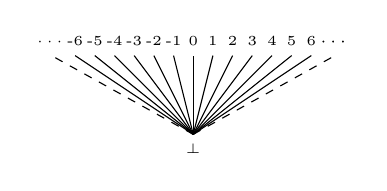
\begin{tikzpicture}
            \draw[dashed, font=\tiny] (0,0) -- (1.8,1) node[above] {$\cdots$};
            \draw[font=\tiny] (1.8,1) node[above] {$\cdots$};
            \draw[font=\tiny] (0,0) -- (1.5,1) node[above] {6};
            \draw[font=\tiny] (0,0) -- (1.25,1) node[above] {5};
            \draw[font=\tiny] (0,0) -- (1.0,1) node[above] {4};
            \draw[font=\tiny] (0,0) -- (0.75,1) node[above] {3};
            \draw[font=\tiny] (0,0) -- (0.5,1) node[above] {2};
            \draw[font=\tiny] (0,0) -- (0.25,1) node[above] {1};
            \draw[font=\tiny] (0,0) node[below] {$\bot$} -- (0,1) node[above] {0};
            \draw[font=\tiny] (0,0) -- (-0.25,1) node[above] {-1};
            \draw[font=\tiny] (0,0) -- (-0.5,1) node[above] {-2};
            \draw[font=\tiny] (0,0) -- (-0.75,1) node[above] {-3};
            \draw[font=\tiny] (0,0) -- (-1,1) node[above] {-4};
            \draw[font=\tiny] (0,0) -- (-1.25,1) node[above] {-5};
            \draw[font=\tiny] (0,0) -- (-1.5,1) node[above] {-6};
            \draw[dashed, font=\tiny] (0,0) -- (-1.8,1) node[above] {$\cdots$};
        \end{tikzpicture}
        \end{center}
    \end{column}
\end{columns}
\end{frame}

\begin{frame}[fragile]
\frametitle{Haskell is non-strict}
\begin{itemize}
    \item \emph{Strict} semantics
          \[
            \forall f: A_\bot \to B_\bot, f(\bot) = \bot
          \]
    \item Non-strict semantics allow operating on (potentially) infinite data
          structures:
          \begin{center}\verb|or ([True] ++ repeat False) == True|\end{center}
    \item Expressions only partially evaluated (\emph{thunks}) until value needed
    \item Problem for effectful computations whose result is never
          needed, e.g.
          \begin{center}\verb|print "Hello, Dave!"|\end{center}
\end{itemize}
\end{frame}

\begin{frame}[fragile]
\frametitle{Haskell is pure}
\begin{itemize}
    \item Functions are mappings from domain to codomain
    \item Haskell functions are \emph{pure}, they are \emph{only} mappings
    \item No side-effects (input/output, changes to global state)
    \item Beneficial for achieving Backus' desiderata
    \item But side-effects are desirable feature of programs
    \item How to bring them back in?
\end{itemize}
\end{frame}

\begin{frame}[fragile]
\frametitle{Computational lambda-calculus and monads}
\begin{itemize}
    \item Eugenio Moggi ('89): program equivalence in $\lambda$-calculus
    \item Semantics for \emph{general} notion of computation
          \begin{itemize}
              \item Side-effects, non-determinism, non-termination
          \end{itemize}
    \item Categorical language semantics with types as objects
          \begin{itemize}
              \item Distinguish type $B$ from corresponding \emph{computations} $TB$
              \item Model each notion of computation as a monad
          \end{itemize}
    \item Adopted into Haskell as general interface to computation
          \begin{itemize}
              \item Functions have to be pure, computations don't
          \end{itemize}
\end{itemize}
\end{frame}

\section{The Category $\Hask$}

\frame{\tableofcontents[currentsection]}

\begin{frame}[fragile]
    \begin{definition}[$\Hask$, intuitively]
        Define the category $\Hask$ to have as objects Haskell types and as
        morphisms $f: a \to b$ pure functions \verb|f :: a -> b|, with
        composition defined by composition in Haskell, $g \circ f :=$
        \verb|g.f| and the identity given as a lambda expression
        \verb|\x -> x|.
    \end{definition}
\end{frame}

\begin{frame}[fragile]
    \begin{itemize}
        \item Haskell implements polymorphic typed lambda calculus
        \item Is $\Hask$ cartesian closed?
        \item Terminals and products from unit type, tuples
        \item Exponentials
        \begin{itemize}
            \item $\texttt{b}^\texttt{a} = \texttt{a -> b}$
            \item $\textrm{eval} = \texttt{uncurry (\$) :: (a -> b, a) -> b}$
        \end{itemize}
        \item But idealization of Haskell required
        \begin{itemize}
            \item Ignore \verb|undefined|, \verb|seq|
            \item Total functions
        \end{itemize}
    \end{itemize}
\end{frame}

\section{Arrows in Haskell}

\frame{\tableofcontents[currentsection]}

\begin{frame}
    \begin{itemize}
        \item Monads take types to computations with result type
        \item No parametrically structured input requirements
        \item \emph{Arrows} as generalizations of computation $X$ to $Y$
        \item Two-parametric, $(X, Y) \mapsto A(X, Y)$
        \item Uniform access to structure on computation input
    \end{itemize}
\end{frame}

\begin{frame}[fragile]
    \begin{definition}[\texttt{Arrow} type class]
        \begin{code}
class Arrow a where
  -- Embed pure computation
  arr   :: (b -> c) -> a b c
  -- Precomposition
  (>>>) :: a b c -> a c d -> a b d
  -- Left-side application
  first :: a b c -> a (b, d) (c, d)

  -- Right-side application (definable)
  (second) :: a b c -> a (b, d) (c, d)
  second f = arr swap >>> first f >>> arr swap

  -- Non-commutative product (definable)
  (***) :: a b c -> a b' c' -> a (b, b') (c, c')
  f *** g = first f >>> second g
        \end{code}
    \end{definition}
\end{frame}

\begin{frame}[fragile]
\begin{definition}[Arrow Laws]
\begin{code}[numbers=left]
              (a >>> b) >>> c == a >>> (b >>> c)
                  arr (g . f) == arr f >>> arr g
                  arr id >>> a == a
                             a == a >>> arr id
           first a >>> arr fst == arr fst >>> a
    first a >>> arr (id *** f) == arr (id *** f) >>> first a
 first (first a) >>> arr assoc == arr assoc >>> first a
                 first (arr f) == arr (f *** id)
               first (a >>> b) == first a >>> first b
\end{code}
Here \verb|assoc| flips tuples \verb|((a,b),c)| to \verb|(a,(b,c))|.
\end{definition}
\end{frame}

\begin{frame}[fragile]
\begin{example}[Pure Functions as Arrows]
\begin{code}
instance Arrow (->) where
    arr f   = f
    f >>> g = g . f
    first f = \symbol{92}(x, y) -> (f x, y)
\end{code}
\end{example}
\end{frame}

\begin{frame}[fragile]
\begin{example}[State Arrows]
\begin{code}
-- Define type
newtype State s x y = ST ((s, x) -> (s, y))

instance Arrow (State s) where
    arr f         = ST (id *** f)
    ST f >>> ST g = ST (g . f)
    first (ST f)  = ST (assoc . (f *** id) . unassoc)

-- A state changing arrow
count :: State Int x y
count = ST ((+1) *** id)
\end{code}
\end{example}
\end{frame}

\section{Freyd categories}

Freyd-categories were introduced by Power \& Robinson~\cite{pow-rob} as a type
of symmetric premonoidal category where the monoidal structure is given by
(the usual) \emph{product} operation. In the paper, this is merely a specific
case of the general notion of symmetric premonoidal categories, which are
proposed as generalisations of monoidal categories for modelling
non-commutative computational effects, such as non-determinism, exceptions and
concurrency.

The actual name, \emph{Freyd-}, is given in a later paper by Power \&
Thielecke~\cite{pow-thie} where Freyd-categories are examined as generalisations
of Cartesian closed categories and closed Freyd-categories are shown to be
models of Moggi's computational $\lambda$-calculus.

It is important to note that, in particular, Power \& Robinson showed that
Freyd-categories generalise strong monads, which were proposed by
Moggi~\cite{moggi-89} as categorical constructs for modelling effectful
computation. Hence the claimed computational-notion generalisations are
directly proved via category theory.

We shall now introduce the necessary notions to describe Freyd-categories and
some basic results about them.

\begin{definition}[Binoidal category]
    A binoidal category is a category $\catC$ equipped with:
    \begin{enumerate}
        \item for each $(A, B)$ in $|\catC| \times |\catC|$, an object $A \otimes B$
            in $|\catC|$;
        \item for each $A$, a functor $(A \rtimes -) : B \mapsto A \otimes B$
        \item for each $A$, a functor $(- \ltimes A) : B \mapsto B \otimes A$
    \end{enumerate}
\end{definition}

The conditions imply that, $A \rtimes B = A \otimes B = A \ltimes B$,
justifying the usage of the notation $A \otimes B$. Observe that this
operation is defined only on objects of $\catC$ so far.

\begin{definition}[Central morphism]
    A morphism $f: A \to B$ in a binoidal category is \emph{central} if for
    every morphism $g: A' \to B'$ the composites of maps (of the form $h
    \ltimes C$ or $C \rtimes h$, where $C$ is either $A$ or $B$ and $h$ is
    either $f$ or $g$) from $A \otimes A'$ to $B \otimes B'$ and from $A'
    \otimes A$ to $B' \otimes B$ agree.
\end{definition}

A natural transformation is central if its components are central.

Having these, we can now define the generalisation of monoidal category.

\begin{definition}[Premonoidal category]
    A \emph{premonoidal category} is a binoidal category equipped with:
    \begin{enumerate}
        \item an \emph{identity object} $I$
        \item for all $A, B, C$, a natural central \emph{associator}
            isomorphism $\alpha_{A,B,C}\colon (A \otimes B) \otimes C \to A
            \otimes (B \otimes C)$
        \item for each object $A$, natural central isomorphisms: \emph{left
            unitor} $\lambda_A\colon A \otimes I \to A$ and \emph{right unitor}
            $\rho_A\colon I \otimes A \to A$
    \end{enumerate}

    such that the usual monoidal category coherence conditions are satisfied,
    i.e.~the pentagon law for $\alpha$ and triangle laws for $\alpha$,
    $\lambda$, $\rho$ hold.

\end{definition}

\begin{example}[Described in \cite{gen-comp-eff-models}]
    Let $\catC$ be a category with finite products and $S$ a specified object
    in $\catC$ (which we regard as \emph{state} or \emph{context}).

    Define $\catx{K}$ as a category such that $|\catx{K}| := |\catC|$ and
    $\catx{K}(X, Y) := \catC(S \times X, S \times Y)$, with composition in
    $\catx{K}$ determined by the composition in $\catC$.

    For any object $X$ of $\catC$, one has evident functors
    $X \otimes -: \catx{K} \to \catx{K}$ and
    $- \otimes X: \catx{K} \to \catx{K}$ extending the product in $\catC$.

    The maps are not bifunctorial (with respect to $\otimes$), hence do not
    yield a monoidal structure on $\catx{K}$. However, they do  yield a
    premonoidal structure on $\catx{K}$.
\end{example}
%% @TODO: grok this example and explain it more.

A \emph{strict premonoidal category} is a premonoidal category in which all the
isomorphisms described above are identities, the $\otimes$ operator is
associative on objects and moreover $I$ is really an identity for $\otimes$.

Note that a strict premonoidal category need not be a monoidal one.

A \emph{symmetric premonoidal category} is a premonoidal category equipped with
a central natural isomorphism $\gamma_{A,B} : A\otimes B \cong B\otimes A$, with
the usual coherence conditions of symmetric monoidal categories.

The \emph{centre} of a premonoidal category $\catC$ is a subcategory $\catC'$,
such that $|\catC| = |\catC'|$ and all the morphisms in $\catC'$ are central.

The centre of a premonoidal category is a monoidal
category~\cite[Prop.~3.1]{pow-rob}.
Hence, a monoidal category is simply a premonoidal category in which all
morphisms are central.

A \emph{strict} (resp. \emph{symmetric}) \emph{premonoidal functor} is a functor which
preserves the strict (resp. symmetric) premonoidal structure and sends central
maps to central maps.

We can now define Freyd categories.

\begin{definition}[Freyd category]
    A Freyd category consists of a category with finite products $\catC$
    and an identity-on-objects strict symmetric premonoidal functor
    \[ J: \catC \to \catx{K} \]
    (hence $\catx{K}$ is a symmetric premonoidal category).
\end{definition}

The definitions of premonoidal categories, and especially Freyd categories,
might seem a bit involved at first sight, however they arise as quite
reasonable generalisations of monoidal categories when one deals with
computational effects. It is hard to phrase this better than one of the
``discoverers'' of Freyd categories, John Power~\cite{gen-comp-eff-models}:

%% @TODO: shorten this and maybe come-up with own motivation / examples
%% if there's time.
\begin{quote}
    The notion of Freyd-category has emerged over the past 15 years as a subtle
    generalisation of the notion of category with finite products. It allows
    one to model environments in call-by-value programming languages containing
    computational effects, notably the $\lambda_c$-calculus, a variant of the
    call-by-value $\lambda$-calculus designed specifically to allow one to account
    for computational effects. Starting with the notion of category with finite
    products, one obtains the notion of a symmetric monoidal category by
    dropping insistence upon the existence of diagonals and projections: in
    such situations, one usually speaks of a tensor product rather than a
    product, corresponding to the relaxation from cartesian logic to linear
    logic. If one further drops the insistence upon bifunctoriality of the
    tensor product, one obtains the notion of a symmetric premonoidal category.
    This corresponds logically to keeping the terms of linear logic but putting
    fewer of them equal.  Just as one has cartesian closed categories and
    symmetric monoidal closed categories, one can speak of closedness for a
    symmetric premonoidal category too. Finally, if one reinstates the
    assumption of finite product structure but only on a specified subcategory
    of a putative symmetric premonoidal category, one has the notions of
    Freyd-category and closed Freyd-category [\ldots]
\end{quote}


\end{document}
